% acmsmall-sample.tex, dated 24th May 2012
% This is a sample file for ACM small trim journals
%
% Compilation using 'acmsmall.cls' - version 1.3, Aptara Inc.
% (c) 2010 Association for Computing Machinery (ACM)
%
% Questions/Suggestions/Feedback should be addressed to => "acmtexsupport@aptaracorp.com".
% Users can also go through the FAQs available on the journal's submission webpage.
%
% Steps to compile: latex, bibtex, latex latex
%
% For tracking purposes => this is v1.3 - May 2012

\documentclass[prodmode,acmtecs]{acmsmall}

% Package to generate and customize Algorithm as per ACM style
%\usepackage[ruled]{algorithm2e}
%\renewcommand{\algorithmcfname}{ALGORITHM}
%\SetAlFnt{\small}
%\SetAlCapFnt{\small}
%\SetAlCapNameFnt{\small}
%\SetAlCapHSkip{0pt}
%\IncMargin{-\parindent}

\usepackage[normalem]{ulem}
\usepackage{epsfig,endnotes}
\usepackage{kotex}
\usepackage{subfig}
\usepackage{comment}
\PassOptionsToPackage{hyphens}{url}
\usepackage[hyphens]{url}
\usepackage{hyperref}
\hypersetup{hidelinks}
\usepackage{multirow}
\usepackage{amsmath}
\usepackage{wasysym}
\usepackage{stmaryrd}
\usepackage{color}
\newenvironment{translatedtext}[2]
   {{\bfseries \color{blue} #1} 
    {\bfseries \color{red}  #2}}

\usepackage{cleveref}
\crefname{section}{§}{§§}
\crefname{section}{§}{§§}

\usepackage{listings}
\lstset{numbers=left, numbersep=5pt, language=C, xleftmargin=12pt}
\usepackage{algorithm}
\usepackage{algorithmicx}
\usepackage{algpseudocode}

% Metadata Information
%\acmVolume{9}
%\acmNumber{4}
%\acmArticle{39}
%\acmYear{2010}
%\acmMonth{3}

\begin{document}

% Page heads
\markboth{J. Yoo et al.}{\texttt{OrcFS}: Orchestrated File System for Flash Storage}

%make title bold and 14 pt font  (Latex default is non-bold, 16 pt) 
\title{\texttt{OrcFS}: Orchestrated File System for Flash Storage} 
\author{Jinsoo Yoo
\affil{Hanyang University}
Joontaek Oh
\affil{Hanyang University}
Seongjin Lee
\affil{Hanyang University}
Youjip Won
\affil{Hanyang University}
Jin-Yong Ha
\affil{Samsung Electronics}
Jongsung Lee
\affil{Samsung Electronics}
Junseok Shim
\affil{Samsung Electronics}}

\begin{abstract}
In this work, we develop OrcFS, \emph{Orchestrated File System} for Flash 
storage. It vertically integrates the log-structured file system and the 
Flash-based storage device eliminating all the redundancies across the 
layers. A few modern file systems adopt sophisticated
append-only data structures to manage its space
in an effort to optimize the behavior with respect to the
append-only nature of the Flash medium.
While the benefit of adopting append-only data structure 
seems to be fairly promising, it makes the stack of software layers full of 
unnecessary redundancies which leaves substantial room for improvement. The 
redundancies include  (i)  redundant levels of indirection  (address
translation) ,  (ii)   duplicate efforts to reclaim the invalid blocks
which is called segment cleaning  and garbage collection in the
file system layer and in the storage device,  respectively, and  (iii)
excessive over-provisioning, i.e.~separate over-provisioning areas in each
layer. OrcFS eliminates the 
redundancies via  distributing the address 
translation, segment cleaning  (or garbage collection), bad block
management, and wear-leveling across the layers.  OrcFS 
consists of three key technical ingredients.
First, OrcFS proposes \emph{Disaggregate Mapping}. OrcFS partitions the Flash storage 
into two areas, each of which is managed by file system and flash storage, 
respectively, with different granularity. In OrcFS, the metadata area and data 
area are maintained by 4 Kbyte page granularity and the 256 Mbyte 
superblock granularity. Second, OrcFS adopts \emph{superblock based storage
management}. It aligns the file system section size which 
is a unit of segment cleaning with the superblock size of the underlying Flash 
storage. We can fully exploit the internal parallelism of the underlying Flash 
storage exploiting the sequenial workload characteristics of the log-structured 
file system.
Third, OrcFS adopts \emph{Quasi-Preemptive Segment Cleaning} to prohibit the foreground 
IO operation from being interefered with excessive segment cleaning overhead. 
The latency to reclaim the free space can be prohibitive in OrcFS.
OrcFS effectively addresses this issue via adopting polling based segment cleaning 
scheme. We develop prototype OrcFS based upon F2FS and server class SSD with modified 
firmware  (Samsung 843TN).
OrcFS reduces the device mapping table requirement to 1/465 and 1/4 compared 
against the page mapping and the smallest mapping scheme known
to public, respectively. 
Via eliminating the redundancy in the segment cleaning and garbage collection, 
the OrcFS removes 1/4 of the write volume under heavy random write
workload. In \emph{varmail}, 
OrcFS achieves 56\% performance gain against EXT4.
\end{abstract}

%%%%%%%%%%%%%%%%%%%%%%%%%%%%
%\category{C.2.2}{Computer-Communication Networks}{Network Protocols}
%\terms{Design, Algorithms, Performance}
\category{D.4.2}{OPERATING SYSTEMS}{Storage Management}
\terms{Design, Management, Performance}

\keywords{Log-structured File System, Flash memories, Garbage Collection}

\acmformat{J. Yoo, J. Oh, S. Lee, Y. Won, J. Ha, J. Lee, and J. Shim,
 2017. \texttt{OrcFS}: Orchestrated File System for Flash Storage}

\begin{bottomstuff}
%This work is supported by the National Science Foundation, under
%grant CNS-0435060, grant CCR-0325197 and grant EN-CS-0329609.

Author's addresses: J. Yoo, J. Oh, S. Lee, and Y. Won, Department of Computer 
and Software, Hanyang University; emails: \{jedisty,na94jun,insight,yjwon\}@hanyang.ac.kr
Ha, J. Lee, and J. Shim, Samsung Electronics; emails: \{jy200.ha,js0007.lee,junseok.shim\}@samsung.com
\end{bottomstuff}
%%%%%%%%%%%%%%%%%%%%%%%%%%%%

\maketitle

\section{Introduction}

Flash based storage device strides its way to main stream storage
medium not only in the mobile device but also in the server and cloud
computing area \cite{enterpriseflash2015berry}. The fraction of Flash
storage sales in the entire storage market has increased from 6.5\% in
2010 to 31.4\% in 2014. It is expected to grow beyond 50\% by the end
of 2016 \cite{3dnand_samsung_news} where most of the growth are from
the server sector. The \$ per byte ratio of SSD against HDD has also
dropped from 6$\times$ in 2012 to 2.8 $\times$ in 2016
\cite{ssdprice}. The rapid proliferation of the Flash storage is
greatly indebted to the introduction of new technology such as 3D-NAND
\cite{3dnand_samsung} and finer process technology \cite{davis2013flash}.

The SSD gets larger and faster. SSD vendors aggressively adopts
internal parallelism, multi-core controller, massive size DRAM.  We
examine the DRAM sizes of 184 SSD models manufactured between 2011 and
2015.
Fig.~\ref{fig:dram_size} illustrates the results. 
The size of DRAM has increased considerably over the years. Mapping
table size roughly equivalent to 0.1\% of the Flash storage
capacity. Our survey reflects this trend. About
60$\%$ of SSDs manufactured recently have 512 Mbyte and 1
Gbyte of DRAM. Despite the sophisticated efforts to increase performance of the SSDs, 
the host is only able to see less than 50\% of the raw bandwidth \cite{sdf}.
Memory overhead soon is going to be   Despite the sophisticated efforts
to harness the SSD with more horse-power, the host is able to see only
less than 50\% of the raw bandwidth \cite{sdf}.

\begin{figure}[t]
\begin{center}
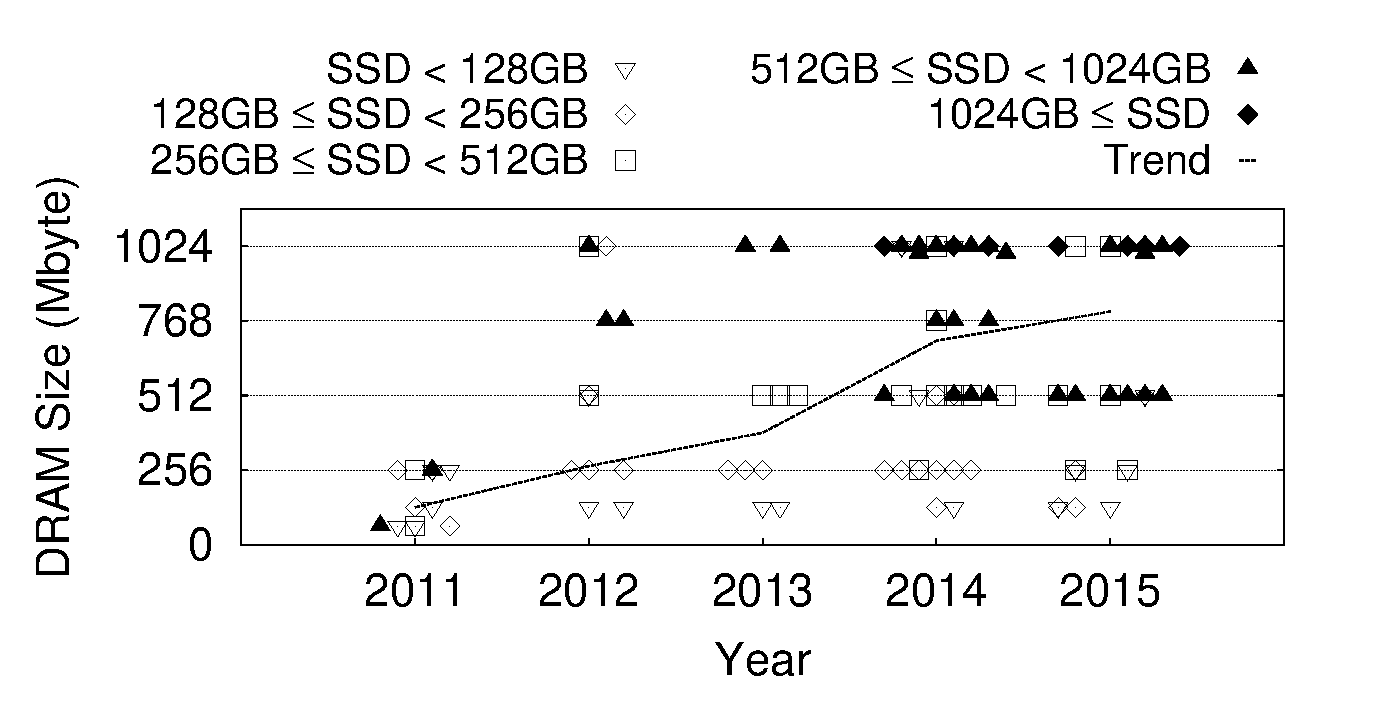
\includegraphics[width=3.6in]{./figure/dram_size.eps}
\caption{DRAM size Trend in SSDs (From 2011 to 2015)}
\label{fig:dram_size}
\end{center}
\end{figure}

The application as well as the file system optimizes itself to better
exploit the physical nature of the underlying Flash storage. The
application adopts write-optimized and append-only search structure
such as LSM-tree \cite{o1996log} in its key-value engine to improve the
insert/update performance \cite{chang2008bigtable,cassandraDB,mongodb,rocksdb}. 
The file systems adopt append-only log structure
in managing its file system partition \cite{lee2015f2fs,nilfs2006} to align its behavior to the
physical nature of the Flash storage. However, these optimization
efforts do not reach far due to the block device abstraction layer
called Flash Translation Layer (FTL) in an SSD  \cite{last08,dftl09,kang2006superblock}. 
Each of the application, file system, and FTL
maintain its own mapping table, perform wear-leveling and garbage
collection, and reserve a fraction of space for over-provisioning
purpose. The redundancies across the layers bring significant waste of
the storage space and duplicate efforts of consolidating the valid
blocks. The redundancies negatively affect the storage performance as
well as the life-span of the storage device.

This work aims at developing a vertically integrated storage stack
eliminating all the redundancies across the layers. We develop
Orchestrated File System, \emph{OrcFS} which directly manages the Flash
blocks. The effort to directly manage to Flash storage is not new. It
dates back to more than a decades ago \cite{woodhouse2001jffs,manning2010yaffs} 
and the new approaches are still being proposed
till today \cite{nvmkv,sdf,anvil,zhangremoving,lee2016application,zhang2016parafs}.
While OrcFS shares much of its philosophy with
the preceding works, it is different in that it intends to directly manage the Flash
storage \cite{lee2016application,zhang2016parafs}. Its actual design
uniquely distinguishes itself from the preceding works in three
aspects; First, OrcFS fully eliminates the redundancy in address
mapping; Second, it fully exploits internal parallelism of the Flash
storage via making the segment cleaning unit of the file system aligned
with the superblock size of the Flash storage; Third, it avoids the
excessive segment cleaning latency due to superblock based cleaning
unit via employing Quasi-Preemptive Segment Cleaning.  We create the prototype
version of OrcFS.  The contributions of this paper are as follows.

\begin{itemize} 
\item {\bf Reduced Memory Overhead:} OrcFS keeps a large mapping unit
  yet without the concerns of block thrashing problem \cite{fast07}. The size of
  memory required to store metadata of an SSD in OrcFS is 1/465 of page
  mapping, and 1/4 of the smallest mapping table size known to the
  public \cite{lee2016application}.

\item {\bf Better Performance and lower write amplification:} OrcFS
enforces append-only write which 
  guarantees that FTL need not have to perform in-place update operations. As the result, the
  performance increases by 50\% and by 21\% against EXT4 under server
  workload (varmail) as well as key-value workload (YCSB).  The write
  amplification in OrcFS is about 26$\%$ lower and IOPS is 45$\%$
  higher compared to that of base F2FS in stacked log-structured
  system.

\item {\bf Elimination of Compound Segment Cleaning:} OrcFS resolves
  compound segment cleaning issue inherent in stacked log-structured
  system. OrcFS sets the unit of segment cleaning same as the unit of
  garbage collection in the storage device. Different partition of the
  storage device is exclusively managed by different layers of the
  storage stack. It entirely eliminates the redundant activity of
  reclaiming invalid blocks across the layer. Since the units on both
  layers are the same, the storage simply can erase the blocks without
  any redundant copies and removes the redundant garbage collection
  overhead between host and the FTL.
\end{itemize}

The rest of the paper is organized as follows.  \cref{sec:background}
describes stacked log system and compound segment collection problem.
\cref{sec:comparison} compares \emph{OrcFS} with other systems.
\cref{sec:OrcFS_design} describes design and implementation of OrcFS.
\cref{sec:experiment} shows the performance of OrcFS through various
experiments and workloads.  \cref{sec:related_works} describes the
related work and \cref{sec:conclusion} concludes the paper.



\section{Background}
\label{sec:background}

\subsection{Segment Cleaning in Log-structured File System}

Log-structured file system is write-optimized file system
\cite{rosenblum1992design}. The file system minimizes seek overhead by
clustering the data block and places the updated metadata blocks in proximity.
The file system writes in an append-only manner and all out-of-date
blocks are marked as invalid. The file system maintains in-memory
directory structure to locate the up-to-date version of individual file
system blocks. To minimize the disk traffic, the file system buffers
the updates and then flushes them to disk as a single unit either when the
buffer is full or when \texttt{fsync()} is called.  The invalid file
system blocks need to be reclaimed to accommodate the newly incoming
writes. The process is called \emph{segment cleaning}. The segment
cleaning overhead is one of the main reasons which barred the wider
adoption of its technology since it makes the file system suffer from
unexpected and long delays \cite{seltzer1995file}.

Append-only nature of the log-structured file system is well aligned
with the update-only nature of the Flash device. A few log-structured
file systems have been proposed specifically for Flash storage
\cite{manning2010yaffs,woodhouse2001jffs,lee2015f2fs}.  However,
Flash optimized file systems still operate on top of block device
abstraction provided by the FTL, and thus, it cannot fully exploit the
raw performance of the SSD \cite{sdf}.


\subsection{Garbage Collection in Flash Storage}

Garbage collection is a process of reclaiming invalid pages in the
Flash storage \cite{agrawal2008design}. Garbage collection not only
interferes with the IO requests from the host but also shortens the
lifespan of the Flash storage. A fair amount of garbage collection
algorithms have been proposed; Greedy \cite{kawaguchi1995Flash},
EF-Greedy \cite{kwon2007ef}, Cost benefit \cite{rosenblum1992design},
etc.  Various techniques have been proposed to hide the garbage
collection overhead from the host. They include background garbage
collection \cite{smith2011garbage}, preemptive garbage collection
\cite{lee2011semi}, etc. SSD controller allocates separate
hardware thread for garbage collection so that garbage collection does
not interfere with IO request from the host.

The host helps FTL to minimize the garbage collection overhead via TRIM command
\cite{shu2007data} and Multi-stream ID \cite{kang2014multi}. Despite
that numerous algorithms have been proposed since the inception of the
Flash storage, the garbage collection is still problematic
\cite{zheng2015optimize,yang2015optimality}.



\subsection{Redundancies Across the Layers}
\label{subsec:stack_logs}

Log-structured file system in its essence is well aligned with the
append-only nature of the SSD. Sequential IO request originated by
log-structured file system can greatly simplify the address mapping
and the garbage collection overhead of the underlying storage.
Recently, a number of key-value stores exploit append-only update
mechanism to optimize its behavior towards write operations
\cite{lim2011silt,ghemawat2014leveldb}.  However, the log-structured
file system for SSD entails a number of redundancies. There are
three major redundancies:  (i)  mapping information,  (ii)  segment
cleaning, and  (iii)  overprovisioning area.
Fig.~\ref{fig:layered_log_system} illustrates an example: a
log-structured file system over an SSD.

\begin{figure}[t]
\begin{center}
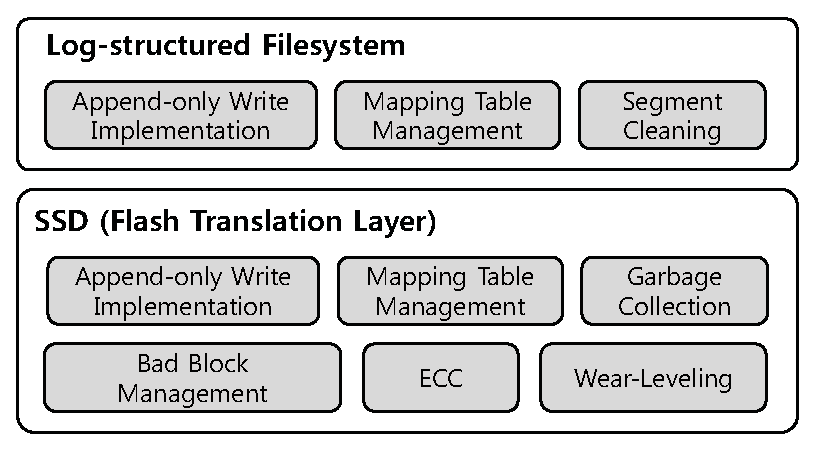
\includegraphics[width=2.8in]{./figure/layered_log_system}
\caption{Log structured file system over Flash storage}
\label{fig:layered_log_system}
\end{center}
\end{figure}

First, each layer has to manage its own metadata for address
mapping. As a result, larger memory is required to load the
metadata. As the capacity of SSD increases, the overhead of
maintaining the mapping information at Flash page granularity becomes
more significant.

Second, each layer performs segment cleaning on its own. We define
compound segment cleaning as the phenomenon where the storage level
log system performs garbage collection on data blocks which are
already segment cleaned by a log-structured file system. The compound
segment cleaning not only degrades the IO performance but also
shortens the lifespan of the Flash storage  \cite{yang2014don,lee2016application,zhang2016parafs}. 

Third, each of the log layers needs to reserve a certain fraction of its
space as the overprovisioning area. The log-structured file system (or
SSD) sets aside a certain fraction of its file system space (or storage
space) to host the extra write operations caused by garbage
collection. Overprovisioning is an indispensable waste of the expensive
Flash storage. The total amount of overprovisioning areas for individual log
layers can be very significant, e.g., 20$\%$ \cite{sdf}. 


\section{Design: Orchestrated File System}
\label{sec:OrcFS_design}


\subsection{Concept}
In this work, we develop Orchestrated File System, \emph{OrcFS}. It
aims at eliminating all data structural and operational redundancies
across the file system and the Flash storage. The address translation
resides either on the host or on the device which is subject to the
file system region. The redundant garbage collection and redundant
overprovisioning are entirely eliminated.  In OrcFS, SSD exposes its
physical blocks to the host and leaves most of its FTL functions
(address translation and garbage collection) to the host
file system. Since the file system is responsible for consolidating the
valid storage blocks, the underlying Flash storage does not have to
set aside a space in the Flash storage for overprovisioning
purposes.

Via eliminating all redundancies, OrcFS reduces the write
amplification, saves space for overprovisioning, and reduces the memory
requirement of the Flash storage device. Eventually, it improves the
performance as well as the life span of the storage device. Also, via
reducing the memory requirement and eliminating the need for
overprovisioning, we can build the Flash storage in much less cost.

\begin{figure}[t]
\begin{center}
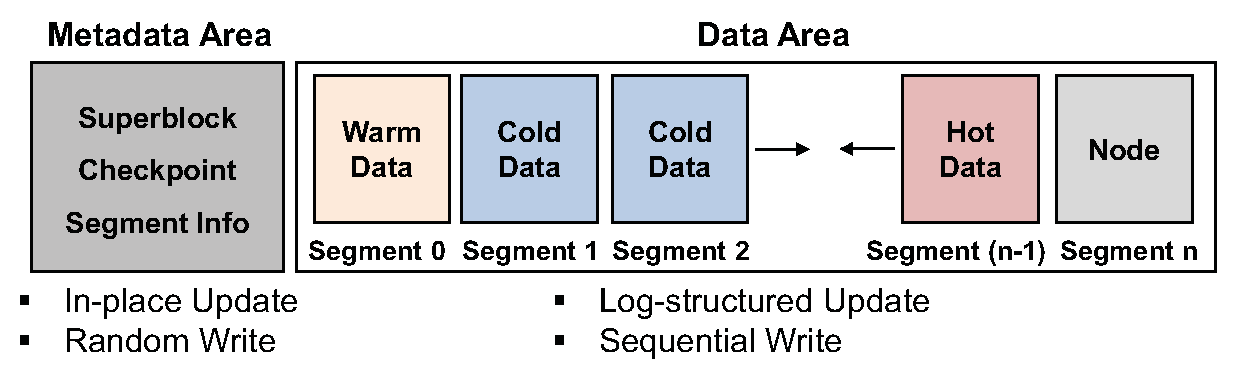
\includegraphics[width=3.4in]{./figure/f2fs_layout}
\caption{F2FS Partition Layout}
\label{fig:f2fs_partition}
\end{center}
\end{figure}

Since the log-structured file system first appeared to public
\cite{rosenblum1992design}, a fair amount of log-structured file systems
have been proposed during the past few decades 
\cite{engel2005logfs,nilfs2006,lee2015f2fs,czezatke2000linlogfs,starwind_lsfs}. While
append-only nature of log-structured file system ideally fits with
the physical characteristics of the Flash storage, most log-structured
file system fail to address the critical issues inherent in
log-structured file system; segment cleaning overhead, \texttt{fsync()}
overhead, and inability to handle direct IO. Due to these reasons, few
works have gone beyond an academic exercises and are used in very
specialized environment \cite{nilfs2006}. Recently proposed F2FS \cite{lee2015f2fs} 
successfully addresses most of the existing issues in
log-structured file system; it properly exploits the append-only nature of the device
and shows good random write performance of Flash storage.


As an initial design choice, we adopt F2FS to manage physical NAND
Flash storage. Instead of clustering the data and the associated
metadata together, F2FS maintains the file system metadata and the
data in the separate region (Fig. \ref{fig:f2fs_partition}).  F2FS
updates the metadata region and the data region in in-place manner and
append-only manner, respectively.  For data region, F2FS categorizes
the data blocks into six categories subject to the file extensions and
access frequency. This greatly improves the efficiency in
consolidating the blocks in the log-structured file system via
clustering the file blocks with respect to their update frequencies.

In OrcFS, the storage blocks in the underlying Flash storage are
partitioned into two regions: Page Granularity Partition and Section
Granularity Partition.  Each of these two partitions occupies
contiguous space in the storage.  The size of these partitions is
aligned with the section size of the F2FS file system.  F2FS provides
a notion of \emph{section}. Section is a set of consecutive file system
segment. Section is a unit of segment cleaning. File system segment
usually corresponds to the NAND Flash block. In OrcFS, each of these
storage partitions is statically bound to the metadata region and the
data region of the file system.

\begin{figure}[t]
\begin{center}
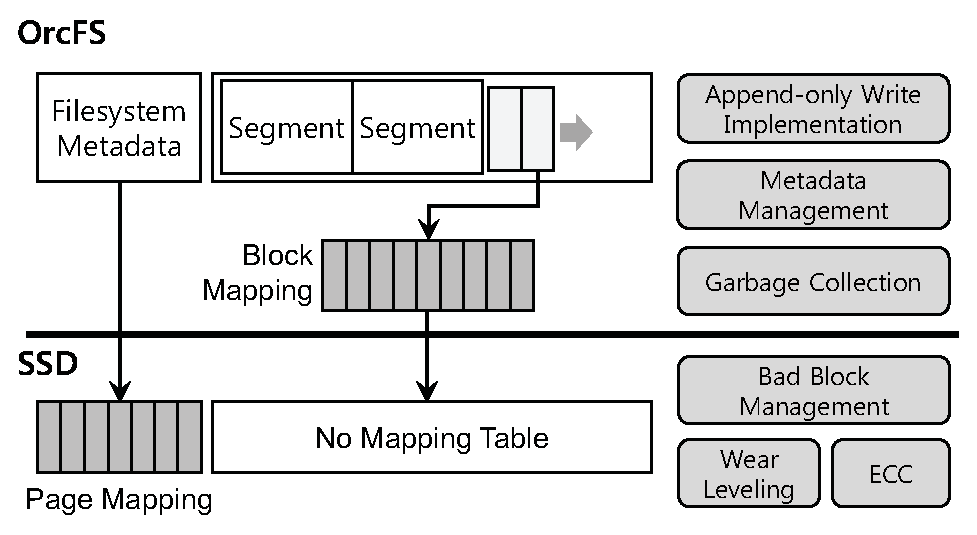
\includegraphics[width=3 in]{./figure/usl_architecture}
\caption{OrcFS Architecture}
\label{fig:usl_layout}
\end{center}
\end{figure}

For metadata region, OrcFS delegates the address translation and its
management, e.g., garbage collection, to the Flash storage. The Flash
storage maintains its own mapping table for the page granularity
partition. For data region, OrcFS is responsible for managing the
physical Flash blocks. When the LBA for an incoming IO requests is for
section granularity region, the Flash storage recognizes the LBA as a
physical address of a flash block and direct the requests to the
respective location.  Fig.~\ref{fig:usl_layout} illustrates the
schematic organization of the OrcFS.

The key ingredients of OrcFS are Disaggregate Mapping and Quasi
Preemptive Segment Cleaning.  We adopt superblock in managing the
data region \cite{park2009sub}.  We develop Quasi Preemptive Segment
Cleaning to minimize the interference of the segment cleaning with
the foreground I/Os.

\begin{figure}[t]
\begin{center}
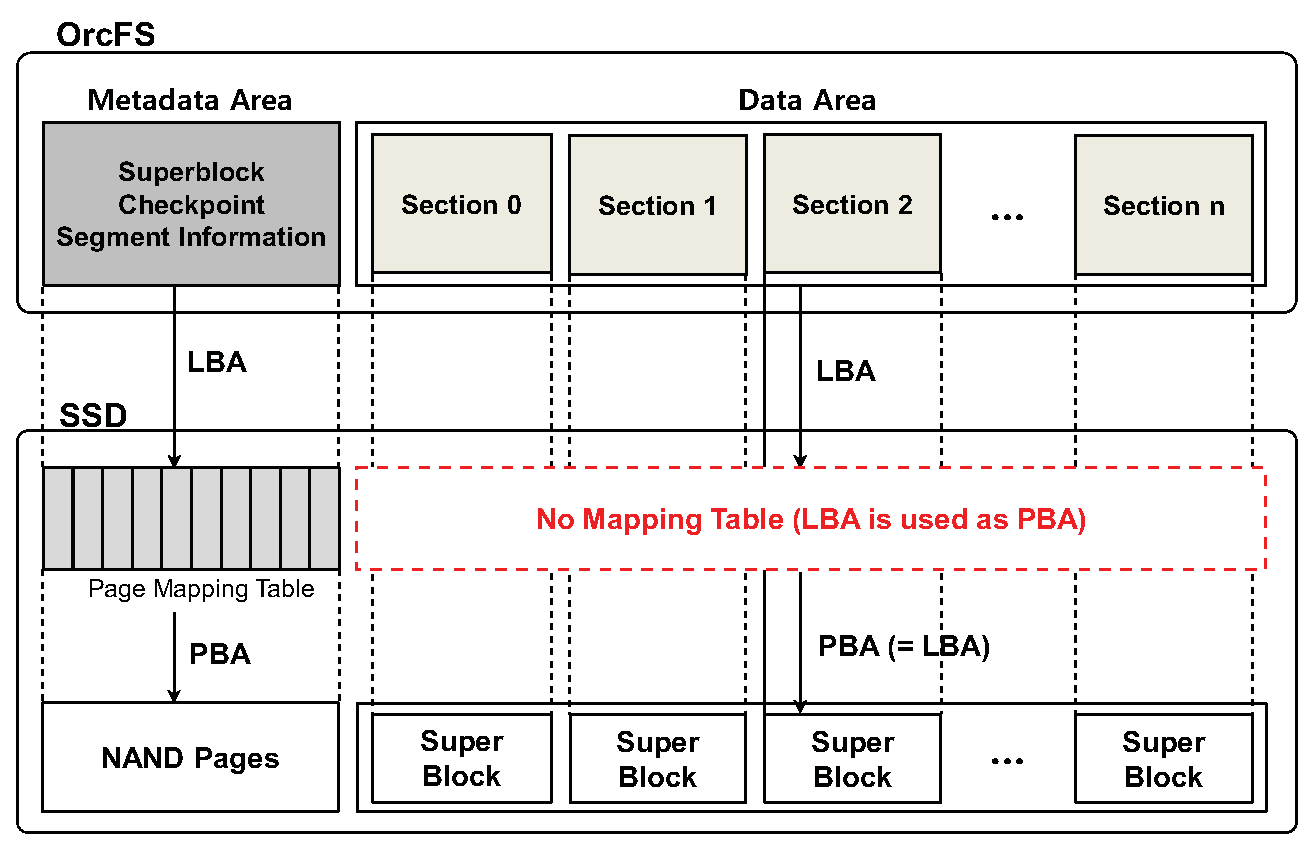
\includegraphics[width=3.6in]{./figure/usl_layout}
\caption{Disaggregate Mapping}
\label{fig:da_mapping_layout}
\end{center}
\end{figure}



\subsection{Disaggregate Mapping}
\label{subsec:da_mapping}

The crux of OrcFS is Disaggregate Mapping. OrcFS manages the two file
system regions, metadata region and data region, differently, both
vertically and horizontally. This mechanism is
called Disaggregate Mapping. The metadata region and data region are managed by
the storage device and the host, respectively. OrcFS applies different
address mapping granularities to each file system partition. It applies
page mapping to metadata region. The data region is
managed by the host file system. The host file system, OrcFS, performs
segment cleaning in the unit of section. The individual sections are
mapped to each superblock in the underlying Flash storage. The unit of
allocation is therefore a superblock. In this regard, the data region is
managed in the superblock granularity. Fig. \ref{fig:da_mapping_layout}
schematically illustrates the Disaggregate Mapping. OrcFS writes to 
metadata region in-place manner, and delegates the address mapping for
this region to Flash storage. OrcFS applies append-only updates to data
region and is responsible for managing it directly. 

The key advantage of OrcFS is superblock unit based storage
management.  Superblock is a set of Flash blocks at the same offset in
the Flash chips from each channel and from each way
\cite{park2009sub}.  Let's consider a 4 channel 2 way SSD. Assuming that a
Flash block is 2 Mbyte, the superblock consists of eight Flash blocks
occupying the same offset from each channel and way combination; thus, the
superblock size corresponds to 16 Mbyte in this example. The file
blocks in a section are consolidated together, and after
consolidation, the entire section becomes free. OrcFS establishes the
size of a section as the size of a superblock. Each file system section
is statically bound to each superblock in the flash storage. This
section-based allocation enables OrcFS to fully exploit the internal
parallelism in the underlying Flash storage leveraging the append-only
sequential write characteristics of the log-structured file system.

Superblock-based management is not without a challenge: inaccurate
block clustering and excessive segment cleaning overhead. Due to its
large size, it is more difficult for SSD firmware to form a superblock
with the Flash pages with similar hotness. In OrcFS, the file system is
responsible for allocating the physical Flash blocks to a given page
cache entries. It classifies a block based upon the block type,
e.g. data block v.s. directory block, or file system extension,
e.g. mp3, mov, etc. OrcFS clusters file blocks together with
respect to the category and hotness and therefore achieves fairly
accurate block clustering \cite{lee2015f2fs,min2012sfs}.  The
overhead of section cleaning will be discussed in the following
section.


The SSD Firmware makes the decision over received LBA. If it is
for metadata area, the firmware directs them to page mapping managed 
region of the device; if LBAs is for the section granularity region, 
the firmware recognizes them as PBAs.

OrcFS successfully eliminates the redundancies in address translation.
Mapping information for metadata area and data area are harbored by
the storage device and the host, respectively.  For 4 Tbyte SSD, the
legacy page mapping requires 4 Gbyte of DRAM for page mapping
table. OrcFS requires only 9 Mbyte at the storage device for mapping
table for metadata region.  While eliminating the redundancy in
address translation looks simple and straightforward, it has profound
implication on the behavior of SSD. It entirely eliminates the
possibility of compound segment collection \cite{yang2014don}.  The
Flash storage is relieved from the burden of allocating surplus
storage space (invisible to the host) for consolidating the valid
blocks.

To guarantee that writes to data area are sequential, we
disabled the threaded logging feature \cite{oh2010optimizations} in
OrcFS.

\subsection{Quasi-Preemptive Segment Cleaning}



Log-structured file system needs to consolidate the valid file system
blocks occasionally. It is called segment cleaning since it creates a
free segment. In OrcFS, the unit of segment cleaning activity is a
section. Due to the large size of a section, the application may
suffer from an excessive delay if I/Os are interfered with the
file system segment cleaning activity. To address this issue, we
develop Quasi-Preemptive Segment Cleaning.

\floatname{algorithm}{Pseudocode}
 \begin{algorithm}[t]
 \caption{Segment Cleaning in OrcFS}
 \label{pseudo:qpsc}
 \begin{algorithmic}[1]
 \small
 \Function{OrcFS\_SegmentCleaning}{$T_{max}$}
 \State lock ($gc\_mutex$)
 \State $T_{start} \gets current\_time()$
 \If{not$\ SC\_context.has\_victim$}
 \State // Get the First Segment Number of the Victim Section
 \State $sec\_no \gets select\_victim\_section()$
 \State $SC\_context.sec\_no \gets sec\_no$
 \State $SC\_context.current\_seg \gets $0
 \Else
 \State $sec\_no \gets $SC\_context.sec\_no
 \EndIf
 \State // Do Segment Cleaning during $T_{max}$
 \State // and check b\_io for Preemption
 \For {offset$\gets$SC\_context.current\_seg to $N_{SegsPerSec}$}
 \State $segment\_cleaning(sec\_no, offset)$ 
 \If{$T_{max} \leq current\_time()-T_{start}$}
 \If{b\_io is not empty}
 \State $SC\_context.has\_victim \gets true$
 \State $SC\_context.current\_seg \gets offset+1$
 \State unlock ($gc\_mutex$)
 \State \Return // Preemption
 \Else
 \State $T_{start} \gets current\_time()$
 \EndIf
 \EndIf
 \EndFor
 \If{this is foreground segment cleaning}
 \State $checkpoint()$
 \EndIf
 \State $SC\_context.has\_vicim \gets false$
 \State unlock ($gc\_mutex$)
 \State \Return
 \EndFunction
 \end{algorithmic}
\end{algorithm}

In segment cleaning, segment cleaning module selects a victim section
and copies the valid file system blocks in the victim section to the
destination section.  It cleans each segment in a section one at a
time. After it cleans all segments in the section, the segment
cleaning module marks the victim section as free.  After then, the
segment cleaning module sends the TRIM command \cite{shu2007data} with
the list of cleaned block numbers as the parameter. The Flash storage
invalidates and erases the associated Flash blocks later in the time
line.

The latency of segment cleaning can be very large. Consider 8 channel
4 way SSD with 2 Mbyte block size. The section size corresponds to 64
Mbyte. Assume that half of the file blocks in a section are
valid. Then, we need to clean two sections to create a new free
section. Copying 64 Mbyte amount of file system blocks entail
significant latency. It can block the application for more than a few
seconds, and the consequence can be disastrous
(Fig. \ref{fig:non_preemptive}).  The existing log-structured
file systems are not designed for this large segment cleaning
unit. While details may vary, the segment cleaning unit establishes an
exclusive lock on the log until it creates a new segment. The
subsequent operation on the respective partition is temporarily
blocked. Let us explain the details.

OrcFS triggers a segment cleaning if the free space in the file system
becomes less than 5\% of the entire file system partition size
(foreground segment cleaning) or if the file system becomes 
idle (background segment cleaning). At the beginning, the segment cleaning
module acquires \texttt{gc\_mutex} lock, which blocks the other
\texttt{kworker} threads from performing write operations till the
lock is cleared. Then, it selects a victim. Foreground
segment cleaning uses greedy \cite{kawaguchi1995Flash} scheme and
background segment cleaning uses cost-benefit
\cite{rosenblum1992design} scheme in victim selection. After selecting
a victim section, the valid blocks in the victim section are read into
page cache. It is worth noting that valid blocks read from the victim
section are categorized as \emph{cold} block \cite{lee2015f2fs}. They
are written to a \emph{cold} segment. In foreground segment cleaning,
the valid blocks are immediately written to the storage creating the
new clean segment. For background segment cleaning, the file system
continues cleaning the next victim segment.  Segment cleaning module
continues to clean the sections until the number of free sections
increases by one. Once it acquires one new free section, the segment
cleaning module flushes the dirty node blocks to the storage and
flushes the file system metadata. Finally, it unlocks the
\texttt{gc\_mutex}.


\begin{figure}[t]
\centering
 \subfloat[Segment Cleaning]{
 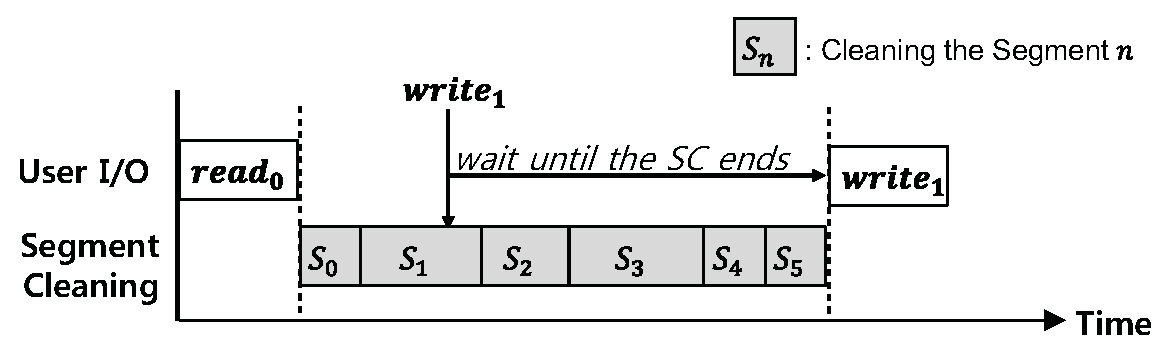
\includegraphics[width=3.6in]{./figure/preemptive_sc_1}
 \label{fig:non_preemptive}
}\hspace{-1.3em}
 \subfloat[Quasi-Preemptive Segment Cleaning]{
 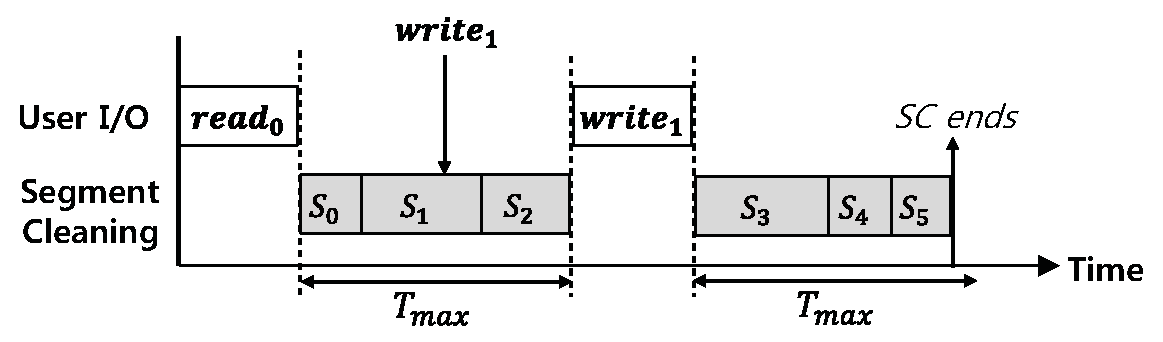
\includegraphics[width=3.6in]{./figure/preemptive_sc_2}
 \label{fig:quasi_preemptive}
}
 \caption{Segment Cleaning}
 \label{fig:quasi_sc}
\end{figure}

The buffered \texttt{write()} system call can be interfered with the
file system segment cleaning. In servicing \texttt{write()}, the F2FS
checks if there is sufficient free space (5\% free space by default in
the storage). If there exist, it allocates a page cache entry for a
given \texttt{write()}. If free space is not sufficient, the
file system triggers segment cleaning. Due to this mechanism, even the
buffered \texttt{write()} can be delayed due to the segment cleaning
mechanism. The application which has issued a \texttt{write()} is
blocked until the segment cleaning ends. The delay can be prohibitive,
especially when the segment cleaning unit is large and when several
segments ( or sections in OrcFS ) need to be cleaned due to high
segment (or section) utilization. 
The \texttt{read()} request is not blocked by the segment cleaning. 
Since \texttt{read()} request does not require a free space in the storage, 
it does not check if there is sufficient free space in the storage nor does 
it wait for the completion of the segment cleaning.

To address this problem, we develop Quasi-Preemptive Segment Cleaning,
\emph{QPSC}. The pseudocode of QPSC is shown in Pseudocode
\ref{pseudo:qpsc}. We define minimum polling interval, $T_{max}$. When
the segment cleaning starts in OrcFS, it sets the timer to
$T_{max}$. After cleaning each segment, the segment cleaning module
examines if the timer has expired. It continues cleaning the segment
if the timer does not expire. If the timer expires, segment cleaning
module examines if there is any outstanding \texttt{write()}
requests. If there exist any pending requests, the segment cleaning
module temporarily releases the lock, \texttt{gc\_mutex()}, and
services the pending requests. After servicing all the pending
requests, the segment cleaning module resumes with the timer reset to
$T\_{max}$. If there is not any pending request, it resets the timer
to $T\_{max}$ and keeps cleaning the segments.

Fig.~\ref{fig:quasi_sc} illustrates 
how the \texttt{write()} request is delayed when it is interfered with
the segment cleaning. In Fig. \ref{fig:non_preemptive}, the
\texttt{write()} is delayed until all the segments, $S_0$, $S_1$,
$\cdots$, $S_5$, in a section are reclaimed. It should be noted that the
\texttt{write()} may have to wait till multiple sections are reclaimed
if the utilization of each section is high. In Fig. \ref{fig:quasi_preemptive}, the \texttt{write()} request is postponed until
the polling interval expires. The \texttt{write()} request is serviced
after reclaiming $S_2$.  The VFS layer of Linux OS maintain a list of
inodes for which there exist outstanding write requests:
\texttt{b\_io} field in the \texttt{bdi\_writeback} structure. The
segment cleaning module examines this list if to determine if there is
any pending requests.


To preserve the context of the segment cleaning, we introduce a new
kernel object, \texttt{SC\_context}. \texttt{SC\_context} maintains
the victim section id, the id of the most recently cleaned segment and
\texttt{has\_victim} flag to determine if these values are
legitimate. The segment cleaning thread starts the cleaning either from
the first segment in the section or from the next segment to the one
stored in the \texttt{SC\_context} subject to the has-victim flag.



\begin{table}[t]
\fontsize{7.5}{10}\selectfont
  \begin{center}
  \begin{tabular}{|c|c|c|c|c|c|c|c|} \hline
  						& OrcFS 			& ParaFS 	& AMF  & NVMKV & ANViL & FSDV & SDF 	\\
  						& 	 			& 2016					& 2016 		& 2015		& 2015 			& 2015		  	& 2014			\\ \hline \hline
%  						& 				& \cite{zhang2016parafs}	& \cite{lee2016application} & \cite{nvmkv} & \cite{anvil} & \cite{zhangremoving} & \cite{sdf}	\\ \hline
  Mapping Table (Host) 	& $\Rightcircle$ 	& $\Circle$				& $\Circle$ 	& $\times$ 	& $\times$ 		& $\times$ 		& $\times$ 		\\ \hline
  Mapping Table (Device) 	& $\Leftcircle$ 	& $\Circle$				& $\Circle$	& $\varocircle$ 	& $\varocircle$ 		& $\varocircle$ 		& $\Circle$ 		\\ \hline
  Device Mapping Table Size			& 2.2 MB	 		& 10 MB					& 8 MB 		& 1 GB 		& 1 GB 			& $\leq$ 1 GB 	& 8 MB			\\ \hline
  Garbage Collection		& Host 			& Host 					& Host 		& Host 		& Device 			& Device 			& Host 			\\ \hline
  Legacy Interface  		& $\Circle$ 		& $\Circle$				& $\times$ 	& $\Circle$ 	& $\times$  		& $\times$ 		& $\times$ 		\\ \hline
  Overprovisioning 		& $\triangle$ 	& $\triangle$ 			& $\times$ 	& $\Circle$ 	& $\Circle$ 		& $\Circle$ 		& $\times$ 		\\ \hline
  Application 			& General 		& General					& General 	& KV Store 	& General 		& General 		& KV Store 		\\ \hline
  \end{tabular}
  \end{center}
    \caption{OrcFS and Other Systems: ParaFS \protect\cite{zhang2016parafs}, AMF \protect\cite{lee2016application}, NVMKV \protect\cite{nvmkv}, ANViL \protect\cite{anvil}, FSDV \protect\cite{zhangremoving}, and SDF  \protect\cite{sdf} (`$\Circle$': medium,
  `$\varocircle$': large, '$\triangle$': small, '$\times$': none,
  Mapping table size is based upon 1 TB SSD with 512 KB Flash block, 4
  KB Page.)} 
  \label{tab:compare_usl}
\end{table}



\subsection{Bad Block Management and Wear-Leveling}
\label{subsec:bad_block_management}

In OrcFS, the storage device is responsible for bad block
management. Bad block management for metadata region is straight
forward since the storage device is in charge of managing the
respective Flash storage partition.  An SSD sets aside a set of NAND
Flash blocks as a spare area \cite{chow2007managing}. There are not
visible to the host.  The mapping unit is aligned with the segment
size, 2 Mbyte.  SSD provides a bad block management module with bad
block indirection table. Bad block indirection table consists of a
pair of $<physical~ block~ number, ~spare~ block~ number>$. Physical
block number denotes the physical block number of the bad block. The
spare block number is the physical block number of the spare block
where the IO request for the bad block is redirected to. In segment
cleaning, all the valid blocks are consolidated to the newly allocated
segment. The replacement block allocated for the bad block is also
migrated to the newly allocated segment. After the replacement block
is copied to the newly allocated segment, the respective bad block
mapping table is reset.  Fig. \ref{fig:bad_block} shows how the bad
block management layer in SSD interacts with segment cleaning.


\begin{figure}[t]
\begin{center}
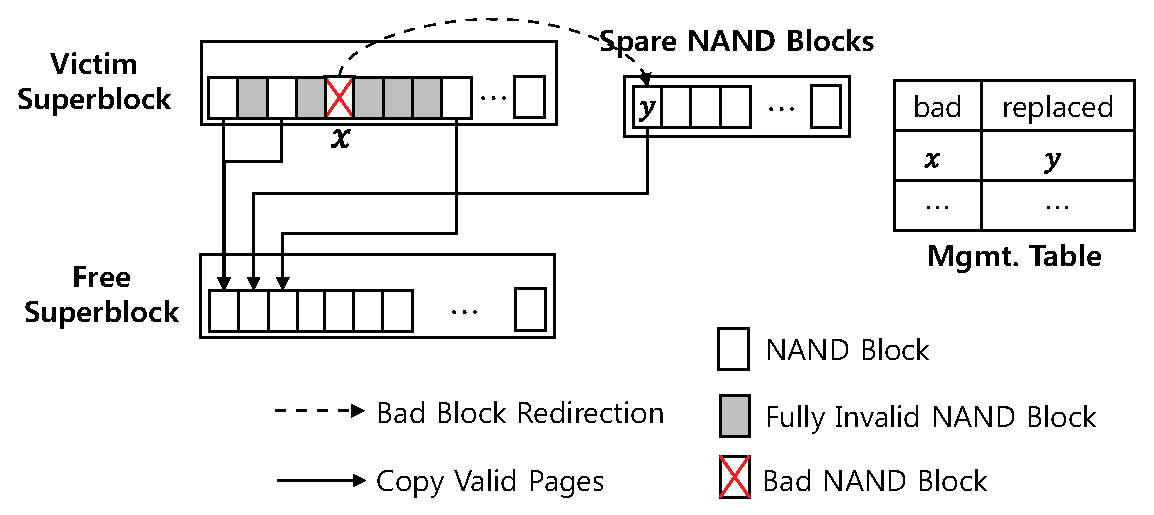
\includegraphics[width=3.6in]{./figure/bad_block_management}
\caption{Segment Cleaning with Bad Block Management}
\label{fig:bad_block}
\end{center}
\end{figure}

There are two approaches in evenly distributing wear of Flash
pages. First, the OrcFS can incorporate the number of wears in
selecting the victim. It can select the sections with the lowest erase
count as the victim section or as a destination section. Second,
the underlying SSD can introduce simple mapping table, and SSD maps the
newly cleaned section to the superblock with the lowest erase count.


\subsection{Implementation Issues}
\label{subsec:OrcFS_implementation}



The file system block size is 4 Kbyte, whereas the page size of an SSD
varies from 4 Kbyte to 16 Kbyte, depending on manufacturers.  In
legacy IO stack, SSD firmware is responsible for handling this
discrepancy through request merge, sub-page mapping, read-modify-write
\cite{agrawal2008design}, etc. In OrcFS, physical Flash pages are
exposed to host and the host file system need to take the
responsibility of resolving this misalignment. We develop \emph{Block
  Patching} for this purpose.

When the write request size is not aligned with the NAND Flash page
size, OrcFS pads free page cache entry (4 Kbyte) to the write request
to make its size aligned with the Flash page size. The file system
needs to allocate additional file system block to accommodate the
padded page cache entry. While the padded page cache entry is not
reflected in the file size, it consumes an additional file system
block.  The patch manager allocates an empty page from the page cache and
concatenates it with the original write request
(Fig. \ref{fig:patch_manager}).  Since a dummy page does not contain
any useful data, we mark it as invalid to let the segment cleaning
module reclaim the page.

In OrcFS, the file system and the storage need to exchange a few
pieces of information; The storage informs the capacity, the Flash page 
size, and the superblock size to the host and the host informs the
storage device about the size of the metadata region. The storage device
uses this information to establish the storage partitions for metadata
region and the data region of the OrcFS file system. Currently, we
implement this feature in the file system format utility,
\texttt{f2fs\_tools} \cite{f2fs_tools}.


\begin{figure}[t]
\begin{center}
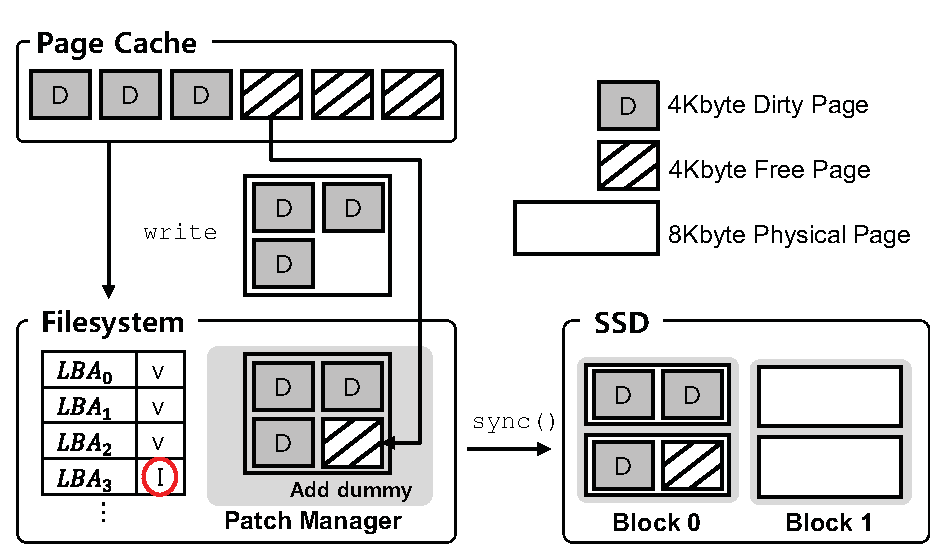
\includegraphics[width=3in]{./figure/patch_manager}
\caption{Block Patching}
\label{fig:patch_manager}
\end{center}
\end{figure}

\section{Comparison}
\label{sec:comparison}
We compare the OrcFS with the six preceding works (Table
\ref{tab:compare_usl}) in the same category where the host directly
manages the device to avoid the redundancies across the layers. ParaFS
\cite{zhang2016parafs} and Application-Managed Flash
\cite{lee2016application} are the closest ones of this sort and use
F2FS to manage the Flash storage. Both of them propose to use block
mapping at the device side to exploit the sequential nature of the
log-structured file system.  The mapping unit is aligned with the
segment size, 2 Mbyte.  There still exists a redundancy in mapping in
these works.  Both the host file system and the storage device
introduce the level of indirection.

NVMKV \cite{nvmkv}, ANViL \cite{anvil} and FSDV \cite{zhangremoving}
use page mapping at the device. ParaFS \cite{zhang2016parafs}, AMF
\cite{lee2016application} and SDF \cite{sdf} use block mapping. For 1
Tbyte SSD, mapping table size corresponds to 1 Gbyte and 8 Mbyte, for
page mapping and block mapping respectively. OrcFS requires only
2.2 Mbytes for the mapping table at the storage device to manage the
metadata region. It only requires 1/4 of the smallest
mapping table in the existing works. There is a critical issue in AMF.
To use only block mapping, AMF modifies the F2FS so that the metadata
region is updated in append-only manner. While this eliminates the
need to manage the metadata region with page mapping, it can cause
cascade updates in the metadata due to the change in the physical
location of metadata \cite{rosenblum1992design}. We suspect that this
brings non-negligible overhead. ParaFS propose to use block mapping (8
Mbyte) and page mapping (2 Mbyte) for data region and metadata region.

Another important aspect is the need to use a special interface. It is
important that the new storage layer is fully functioning without any
changes in the existing applications and does not need any special
interface. Among seven works in Table \ref{tab:compare_usl}, only
OrcFS, ParaFS, and NVMKV are compatible with standard API.


The size of the mapping table in FSDV is dynamically resized, and in
the worst case, the size of the mapping table becomes the same size as
a page mapping table.  NVMKV \cite{nvmkv} removes the host-side
metadata and leverages FTL metadata and interfaces to manage the
key-value store.  NVMKV still requires a page granularity mapping table
in the device.  Also, NVMKV \cite{nvmkv} and SDF \cite{sdf} are limited to
a specific workload such as a key-value store.

ANViL \cite{anvil} lets the host modify device logical-to-physical
mapping information through a new I/O interfaces, but mapping table
overhead is still significant.

Summarizing all this, we carefully believe that the benefit of OrcFS
is clear.


\section{Experiment}
\label{sec:experiment}

\subsection{Experiment Setup}
\label{subsec:exp_setup}

We compare the performance of OrcFS against F2FS and EXT4 on Linux
Kernel 3.18.1. OrcFS uses disaggregate mapping, and F2FS and EXT4 use
page mapping SSD.  We used Samsung SSD 843Tn \cite{ssd843tn} for
experiments, and modified its firmware to implement OrcFS.  To use
disaggregate mapping on the device, we disable SSD garbage collection
in the data area, and use the information given by the
\texttt{mkfs.f2fs} to bind the logical address to the physical
address. The firmware manages metadata area with page mapping. It
performs garbage collection on only metadata area.


Table \ref{tab:ssd_info} shows the specification of the host system
and SSD 843Tn used in the experiment. The superblock size is 256
Mbyte.

Since F2FS exhibits the best performance when the size of the section
matches the garbage collection unit of the storage device, we set the
section size of F2FS to 256 Mbyte in all experiment.  We checked the
performance of F2FS while varying the size of a section.  Compared to
the IOPS and WAF of F2FS with section size of 2 Mbyte, F2FS with
section size 256 Mbyte shows 24$\%$ higher IOPS and 20$\%$ lower WAF.


\begin{table}[t]
\begin{center}
\begin{tabular}{|c|p{3cm}|p{3cm}|} 			\hline
			& Desktop			& Server		\\ \hline\hline
		CPU	& Intel i7-3770	& Xeon E5-2630 \\ \hline
		Mem	& 8 GB			& 256 GB 		\\ \hline
		OS	&	\multicolumn{2}{c|}{Ubuntu 14.04 (kernel 3.18.1)} \\ \hline
\multirow{2}{*}{Storage}	& \multicolumn{2}{c|}{Capacity: 256 GB (include 23.4 GB OVP)}  \\ 
						& \multicolumn{2}{c|}{4 MB NAND Block size, 8 KB Page size}  \\ \hline
\end{tabular}
\end{center}
\caption{Host system and Storage (Samsung SSD 843Tn \protect\cite{ssd843tn})}
\label{tab:ssd_info}
\end{table}


\begin{table}[t]
\begin{center}
\begin{tabular}{|c|c|c|c|c|c|} \hline
  		     & Files	& File size & Threads & R/W   & fsync 		\\ \hline\hline
  fileserver	& 80,000	& 128 KB	   & 50	    & 33/67 & N\\ \hline
  varmail 	& 8,000	& 16 KB     & 16	    & 50/50 & Y\\ \hline
\end{tabular}
\end{center}
%\vspace{-0.7em}
\caption{Summary of Filebench Workload}
\label{tab:filebench}
\end{table}

\begin{table}[t]
\begin{center}
  \begin{tabular}{|c|r|} \hline 
                         & Mapping Size       \\ \hline\hline 
Page mapping             & 256 Mbyte          \\ \hline 
FSDV \cite{zhangremoving} & $\leq$ 256 Mbyte  	\\ \hline 
Hybrid mapping \cite{last08} & 4 Mbyte \\ \hline 
Disaggregate Mapping     & 1 Mbyte            \\ \hline
\end{tabular}
\end{center}
%\vspace{-0.7em}
\caption{Size of Mapping Table (256 Gbyte SSD)}
\label{tab:meta_size}
\end{table}

\subsection{Mapping Table Size}

Table \ref{tab:meta_size} compares the size of mapping tables in Page
mapping, FSDV \cite{zhangremoving}, Hybrid mapping \cite{last08}, and
Disaggregate mapping.  Page mapping uses 256 Mbyte of memory when
disaggregate mapping of OrcFS uses only 1 Mbyte. As the size of SSDs
is increasing, the mapping table overhead becomes significant.  For 1
Tbyte and 4 Tbyte SSD with 4 Kbyte as the page size, the memory space
required to store the mapping table information is 1 Gbyte and 4
Gbyte, respectively.

File System De-Virtualizer, FSDV \cite{zhangremoving}, makes file
system point to a physical address in an SSD, and the pointed entry in
the SSD is removed from the mapping table. The size of the mapping
table is dynamically resized. In the worst case scenario, it has to
maintain 256 Mbyte of the mapping table, just like the page mapping
table.

The memory footprint of OrcFS is only 1 Mbyte which consumes
about 256 times less than that of page mapping. Even if we add several
other metadata used by OrcFS, such as segment bitmap and buffered
segment number, the size of total metadata is only 4.73 Mbyte, which
is 54 times less than that of page mapping. LAST FTL consumes is 4 Mbyte
for mapping table.


\begin{figure}[t]
\centering

 \subfloat[Sequential Write]{
 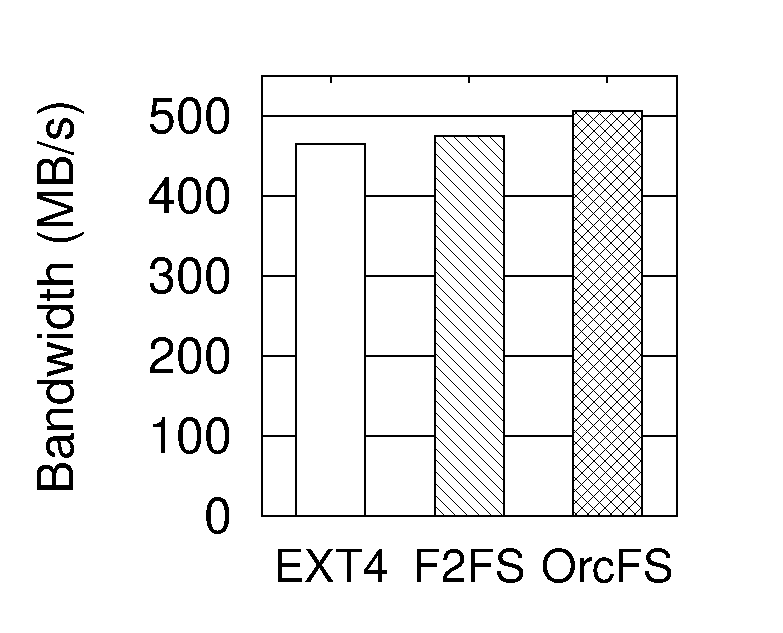
\includegraphics[height=1.5in]{./bench/seq_write}
 \label{fig:benchtest_seqw}
}
 \subfloat[Random Write]{
 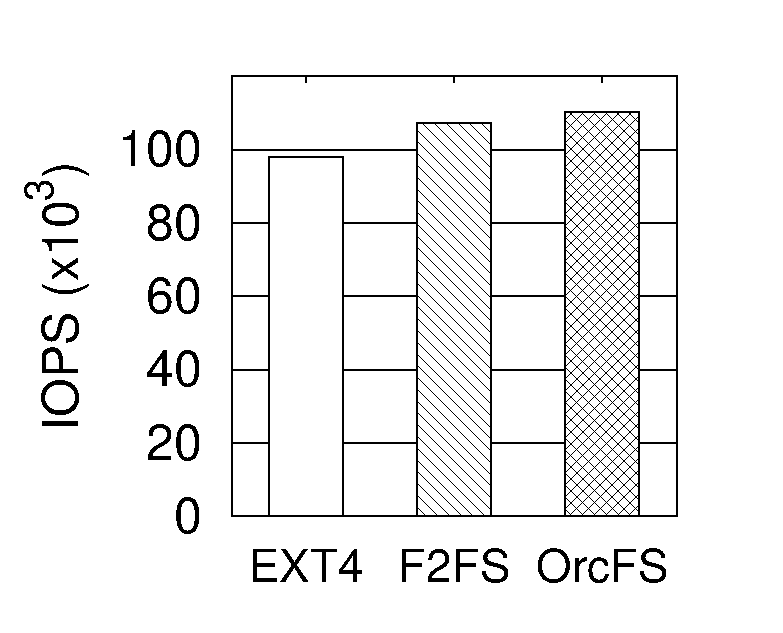
\includegraphics[height=1.5in]{./bench/rand_write}
 \label{fig:benchtest_randw}
}
 \caption{Sequential / Random Write Performance. Sequential Write: 188
   Gbyte File size, 512 Kbyte record size, 2.75 Tbyte Total write
   volume / Random Write: 50 Gbyte File size, 4 Kbyte record size, 750
   Gbyte Total write volume, Section size of F2FS: 256 Mbyte}
 \label{fig:benchtest}
\end{figure}


\subsection{Primitive IO}
\label{subsec:io_performance}


We measure the performance of sequential write and random write
(Fig. \ref{fig:benchtest}).  We format the file system and create a
file with a size of 188 Gbyte. One iteration of an experiment issues
512 Kbyte buffered sequential write until all LBAs are overwritten. We
repeat the iteration for fifteen times.  Fig. \ref{fig:benchtest_seqw}
shows the average performance. The performance of EXT4 and F2FS is 466
Mbyte/sec and 476 Mbyte/sec, respectively. The performance of OrcFS
shows about 507 Mbyte/sec. It is 6$\%$ higher than that of F2FS.

The performance gap between EXT4 and OrcFS stands out more in random
write workload (Fig. \ref{fig:benchtest_randw}).  To measure the
random performance of the device, we format the device and create a 50
Gbyte sized file in the partition. An iteration of the experiment
touches all the LBAs with 4 Kbyte buffered random writes, and the
graph shows the average of fifteen iterations. OrcFS is 12$\%$ faster
than EXT4; IOPS of OrcFS is 110.3 KIOPS and Ext4 is 98.1 KIOPS.


\begin{figure}[t]
  \begin{center}
  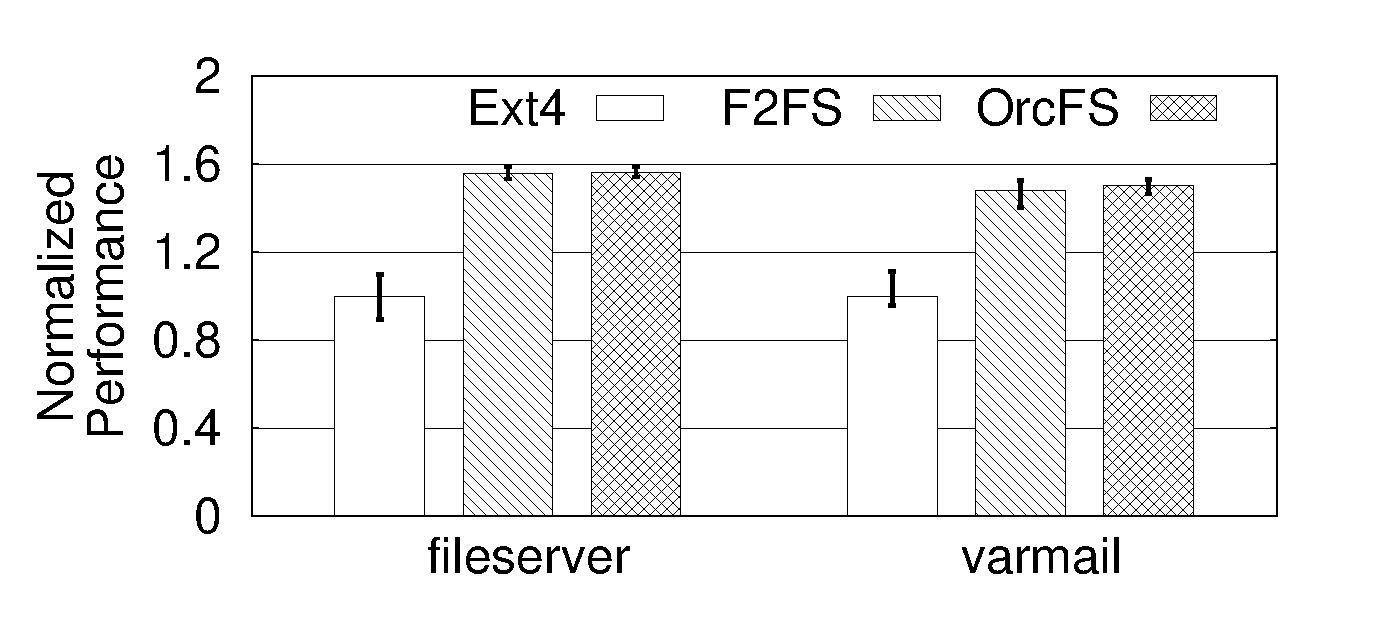
\includegraphics[height=1.5in]{./bench/filebench.eps}
  \caption{Filebench}
  \label{fig:filebench}
  \end{center}
\end{figure}

\begin{table}[t]
\begin{center}
\begin{tabular}{|c|c|c|c|c|c|} \hline
  		& 25\%	& Median	& Mean	& 75\%   \\ \hline\hline
  EXT4	& 4 KB	& 12 KB	& 120 KB	& 212 KB \\ \hline
  F2FS 	& 304 KB	& 424 KB	& 360 KB	& 480 KB	\\ \hline
  OrcFS 	& 312 KB	& 432 KB	& 365 KB	& 488 KB 	\\ \hline
\end{tabular}
\end{center}
%\vspace{-0.7em}
\caption{SATA write request size (filerserver)}
\label{tab:fileserver_size}
\end{table}

\subsection{Macro Benchmark}
\label{subsec:micro_bench}

We use two workloads; fileserver, varmail from Filebench
\cite{filebench}.  Table \ref{tab:filebench} shows the summary of the
each filebench workload.  \emph{fileserver} workload generates 80,000
files with a size of 128 KByte, then creates 50 threads to issue reads
or buffered appends with the ratio of 33:67. In the fileserver
workload, on the average the size of append requests is 16 Kbyte.
\emph{varmail} creates eight thousand 16Kbyte files using 16 threads
to create and delete the files with ratio of 50:50, and each operation
is followed by \texttt{fsync()}.



Fig. \ref{fig:filebench} shows the result of filebench
\cite{filebench} using \emph{fileserver} and \emph{varmail} workload.
The performance is normalized with respect to the performance of EXT4.
In the case of fileserver workload, OrcFS shows 60$\%$ higher
performance than EXT4.  We examine the details. Table
\ref{tab:fileserver_size} shows the quartile statistics of the size of
writes in the fileserver workload.  The median of write request size
of OrcFS, 432 KByte, is about 36 times larger than that of EXT4, 12
Kbyte. The log-structured file system merges the received write
requests into larger one before dispatching them to the storage.  The
number of write requests in OrcFS is about the half of the number in
EXT4 (119,482).


The result is similar in varmail workload. It shows that the
performance of OrcFS is 50$\%$ better than that of EXT4 (20
Mbyte/sec). EXT4 shows slower performance than the other two file
systems because EXT4 sends a lot of \texttt{discard} commands to inform
the state of the deleted file blocks to the storage device. While the
way to handle discard command vary by the SSD vendors, it needs to
invalidate the mapping table entry for the deleted file blocks and can
accompany non-negligible overhead \cite{saxena2010flashvm}.  F2FS and
OrcFS also issue the \texttt{discard} command.
However, the overhead is not as significant as in the case of EXT4
because a much smaller number of discard commands are being issued.



\subsection{Key-Value Store Workload}
\label{subsec:ycsb_bench}

\begin{figure}[t]
  \centering
   \subfloat[Throughput]{
   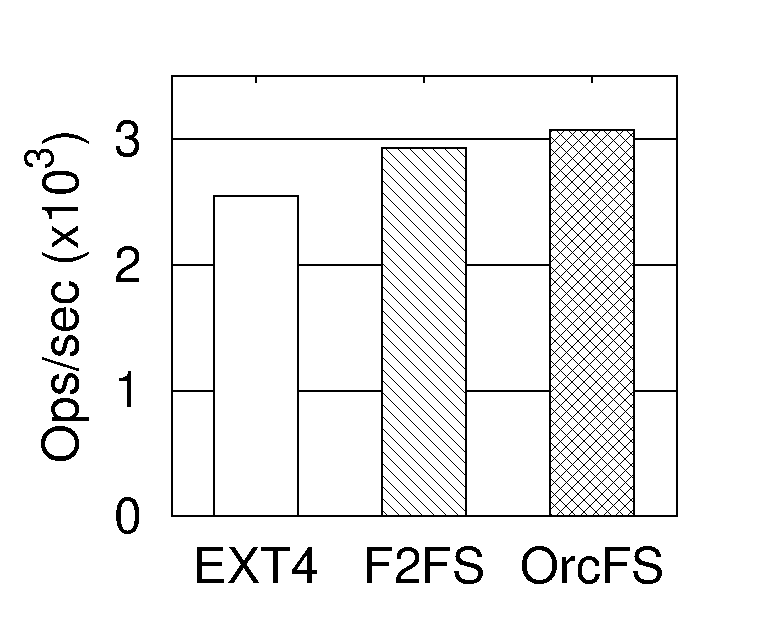
\includegraphics[height=1.4in]{./bench/ycsb_throughput.eps}
   \label{fig:ycsb_throughput}
  }
   \subfloat[Update Latency]{
   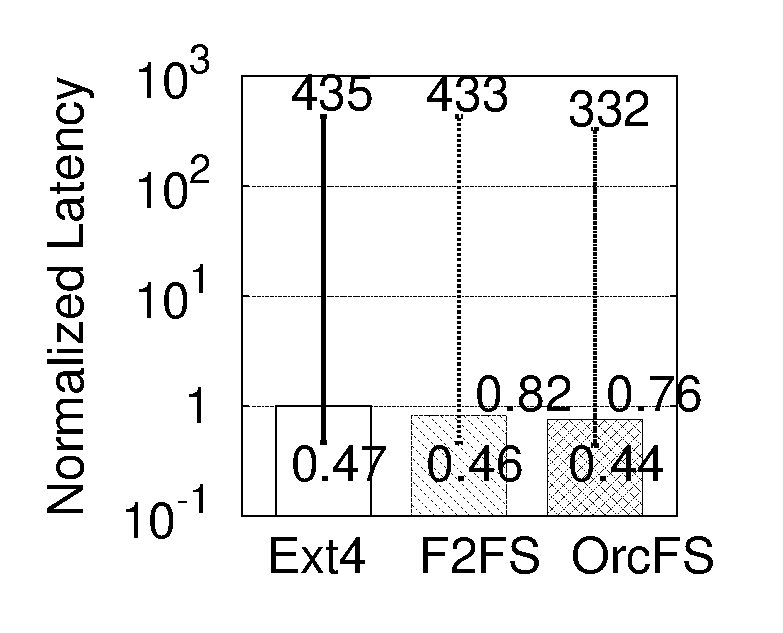
\includegraphics[height=1.4in]{./bench/ycsb_latency.eps}
   \label{fig:ycsb_latency}
   }
   \caption{Cassandra (YCSB)\label{fig:ycsb}}
\end{figure}

We use Cassandra DB \cite{cassandraDB} with YCSB to measure the
performance of EXT4, F2FS, and OrcFS. Cassandra DB adopts
log-structured merge tree \cite{o1996log} as its essential data
structure.  The size of the DB used in the experiment is 20 Gbyte.  We
used YCSB Workload-A to perform read and update operation with the
ratio of 50:50.

\begin{comment}
\begin{table}[t]
\begin{center}
\begin{tabular}{|c|c|c|c|c|c|} \hline
  		& 25\%	& Median	& Mean	& 75\%   \\ \hline\hline
  EXT4	& 16 KB	& 512 KB	& 360 KB	& 512 KB \\ \hline
  F2FS 	& 512 KB	& 512 KB	& 413 KB	& 512 KB	\\ \hline
  OrcFS 	& 512 KB	& 512 KB	& 418 KB	& 512 KB 	\\ \hline
\end{tabular}
\end{center}
%\vspace{-0.7em}
\caption{SATA write request size (run phase)}
\label{tab:ycsb_run}
\end{table}
\end{comment}

Fig. \ref{fig:ycsb_throughput} shows the overall throughput of
read/update operation. The throughput of OrcFS (3,145 Kops/sec) is
about 21$\%$ and 15$\%$ higher than that of EXT4 and F2FS,
respectively. Fig. \ref{fig:ycsb_latency} shows the normalized latency
of update operation of each file systems against EXT4. The latency in
OrcFS is about 24$\%$ lower than the EXT4.

We perform detailed analysis to identify the cause for this
performance discrepancy.  We examine the number of write commands and
the number of synchronous writes in systems.  EXT4 had the most number
of SATA write commands and the synchronous writes. EXT4 generated
20$\%$ more write commands than that of OrcFS.



\begin{figure}[t]
  \centering
   \subfloat[w/o QPSC]{
   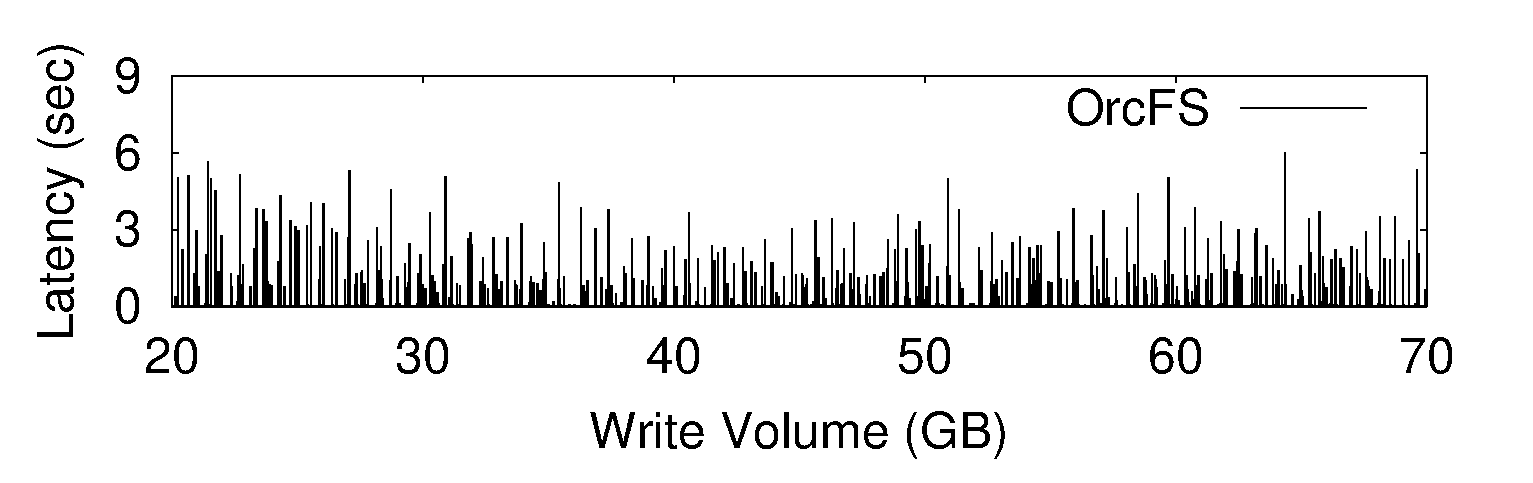
\includegraphics[width=3.5in]{./qpsc/normal_latency.eps} 
   \label{fig:lat_wo_qpsc}
   }\quad 
   \subfloat[w/ QPSC]{
   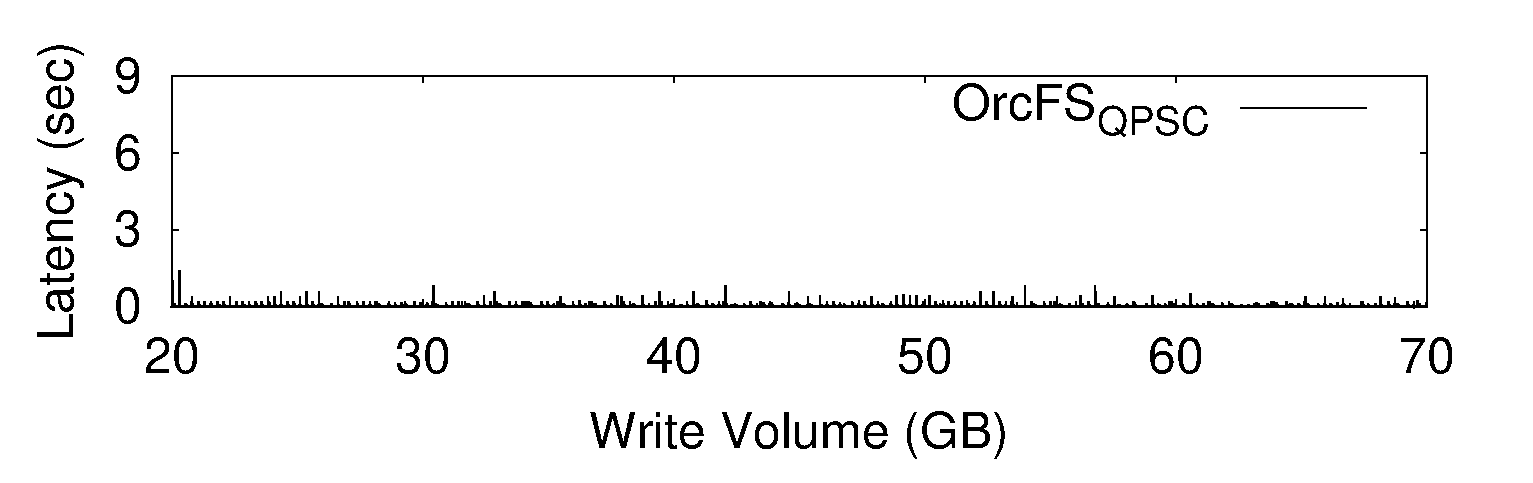
\includegraphics[width=3.5in]{./qpsc/qpsc_latency.eps}
   \label{fig:lat_w_qpsc}
   }
   \caption{Write Latency (110 Gbyte Cold File, 80 Gbyte Hot File, 4
     KByte Buffered Random Write to Hot File)\label{fig:lat_qpsc}}
\end{figure}

\begin{comment}
\begin{table}[t]
  \begin{center}
  \begin{tabular}{|c|c|c|c|c|c|} \hline
   				& Avg 		& 99\%	& 99.9\% 		& 99.99\% 	& Max 	\\ \hline\hline
  OrcFS			& 44 us		& 11	us	& 36 us		& 21 ms		& 8.9 sec	\\ \hline
  OrcFS$_{QPSC}$	& 43 us		& 10	us 	& 11 ms		& 70 ms 		& 1.4 sec	\\ \hline
  \end{tabular}
  \end{center}
  \caption{Quartile Information of Write Latency (us: microsecond, ms: millisecond)}
  \label{tab:qpsc_latency}
\end{table}
\end{comment}

\subsection{Quasi-Preemptive Segment Cleaning}
\label{subsec:qpsc_test}

We examine the effect of segment cleaning over the latency of
foreground IO. We perform 4 Kbyte buffered \texttt{write()} and create
a situation where there runs out of the free section.  When there runs out
of the free section, the segment cleaning module of both F2FS and OrcFS
cleans the sections until it creates at least one additional
section. If the section utilization is $\rho$, it needs to clean
$\frac{1}{1-\rho}$ sections to create one additional free sections.
If $\rho$ is 0.6, the segment cleaning module consolidates the blocks
from at least three sections. With 256 Mbyte section, it has to scan
800 Mbyte of file system blocks and migrates nearly 600 Mbyte of data
blocks to a destination section. If this operation interferes with the
ongoing IO, the application may experience an intolerable amount of
delay. We examine the latency of 4 Kbyte buffered write() operation.

We set the polling interval to 100 m sec.  Fig. \ref{fig:lat_qpsc}
illustrates the result.  We only show the interval where the segment
cleaning is active. As can be seen, without proper management, the
latency of 4 Kbyte write() can be as high as 9 sec. It is
prohibitive. With 100 m sec polling interval in Quasi Preemptive
Segment Cleaning, we cannot observe any abnormal delay which has been
observed in F2FS. In OrcFS, the latency of write operation is less
than one sec.  Quasi-Preemptive Segment Cleaning successfully resolves
the excessive segment cleaning overhead which may appear in large size
section based space management.

\begin{comment}
  \begin{table}[t]
  \begin{center}
  \begin{tabular}{|r|r|r|r|r|r|} \hline
  	     	& Min	& Avg 		& 99.9\% 		& Max 		\\ \hline\hline
  OrcFS	(msec)    		& 15.6 & 929.2 & 5,734.6 & 6,651.9 	\\ \hline
  OrcFS$_{QPSC}$ (msec)	& 1.2 & 111.3	& 252.6 & 278.4	\\ \hline
  \end{tabular}
  \end{center}
%  \vspace{-0.7em}
  \caption{OrcFS Segment Cleaning Latency according to Quasi-Preemptive Segment Cleaning (msec)}
  \label{tab:lat_qpsc}
  \end{table}
\end{comment}

\subsection{Effect of Eliminating the Redundancies}
\label{subsec:remove_gc_overhead}

OrcFS eliminates the redundancies in the address translation across 
the layers. Different regions of the storage are managed by different 
layers of the storage stack: data region by the host file system and the 
metadata region by the storage device, respectively. The benefit is 
clear. There will be no compound storage consolidating effort. We measure 
the effectiveness of eliminating the redundancies from the perspective of 
write amplification as well as from the perspective of the performance. 
The workload is carefully crafted to trigger the garbage collection at 
the storage device as well as at the segment cleaning at the file system. 

The garbage collection and the segment cleaning behavior is governed by 
the free space at the file system, the size of the overprovisioning area 
at the Flash storage, For 256 GByte SSD, we create 170 Gbyte file. For 
170 GByte file, we designate the half of the file as the hot region. We  
perform random write only to the hot region of the file. A single iteration 
ends if all blocks are over-written. Random writes (buffered 4 Kbyte write) 
are created so that each of the file blocks in the hot region is written 
one and only once. We run the fifteen iterations of this workload. Write 
amplification is measured using \texttt{smartmontools} \cite{smartmontools}.

\begin{figure}[t]
  \centering
  \subfloat[WAF]{
    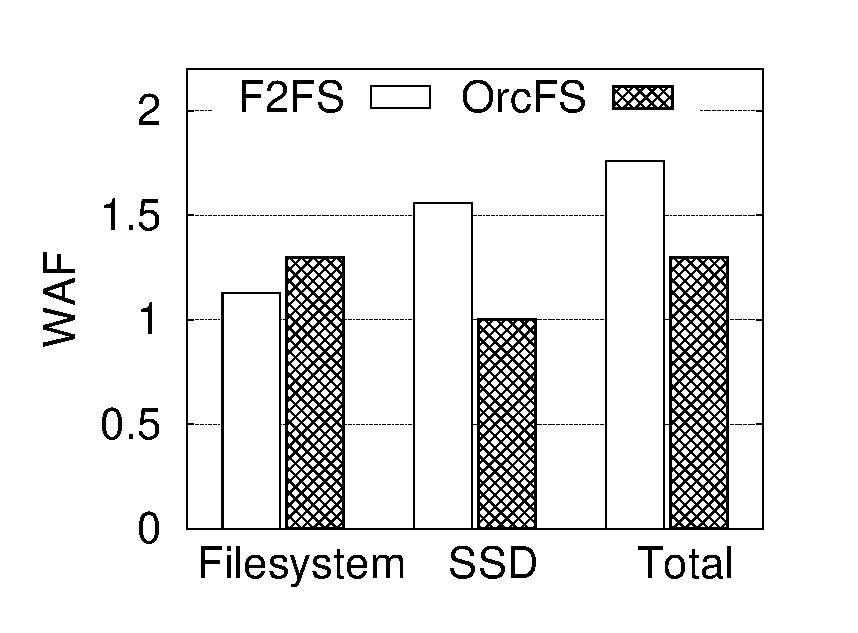
\includegraphics[height=1.6in]{./comp_gc/f2fs_vs_usl_waf}
   \label{fig:f2fs_vs_usl_waf}
  }
   \subfloat[IOPS]{
   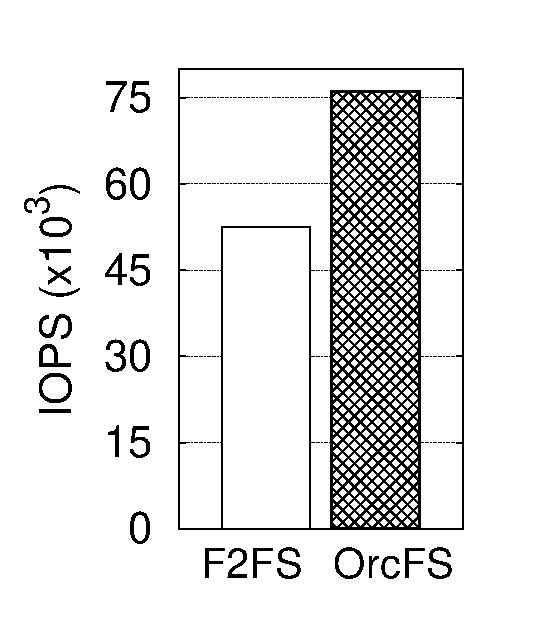
\includegraphics[height=1.6in]{./comp_gc/f2fs_vs_usl_iops}
   \label{fig:f2fs_vs_usl_iops}
  }
   \caption{WAF and IOPS of Each System  (85 Gbyte Cold File, 85 Gbyte
     Hot File, 4 Kbyte buffered random write to the Hot File, 170
     Gbyte Total write volume, Section size of F2FS: 256
     Mbyte) \label{fig:f2fs_vs_usl}}
\end{figure}

First, we examine the performance. F2FS and OrcFS yield 53K IOPS and
75K IOPS, respectively (Fig. \ref{fig:f2fs_vs_usl_iops}). OrcFS shows
45\% performance gain against F2FS. Second, we examine the write
amplification created by each layer. Fig. \ref{fig:f2fs_vs_usl_waf}
illustrates the result. In the file system level, F2FS and OrcFS
amplify the write by 1.13 and 1.3, respectively. Due to the larger
segment cleaning unit size, it is inevitable that OrcFS inefficiently
consolidates the file blocks and therefore has larger write
amplification. SSD in F2FS and SSD in OrcFS exhibit a stark contrast in
write amplification. In F2FS, the underlying SSD amplifies the write
operation by 1.56. This is due to garbage collection in the storage
device. On the other hand, in OrcFS, since the file system is in charge
of consolidating the physical NAND flash storages, the storage device
itself does not entail any amplification.  The segment cleaning at the
file system and the garbage collection at the storage device
compounds. F2FS and OrcFS yields 1.76 and 1.3 write amplification seen
from the storage device. OrcFS eliminates 1/4 of the write volume.

Third, we analyze the cause for this
amplification. Fig. \ref{fig:io_distribution} illustrates the
result. The application creates 85 GByte of write to the file system
data region in both F2FS and OrcFS. In F2FS and OrcFS, the file system
creates 431 Mbyte and 599 Mbyte of metadata update, respectively.  The
reason that OrcFS updates more metadata than that of F2FS is because
OrcFS writes only in append-only style, whereas F2FS exploits threaded
logging \cite{lee2015f2fs} to reduce the number of segment cleaning
when the file system utilization is high. On top of that, dirty data
in node segments also has to be flushed to the storage at the time of
checkpoint which is called at the end of a segment cleaning.  In F2FS,
we observe that Flash storage creates a huge amount of writes by itself
due to garbage collection. Meanwhile, OrcFS is free from this behavior
yielding much more efficient storage behavior.

The write volume governs the lifespan of the Flash storage. Roughly,
eliminating the 1/4 of total write volume lead to the 30\% extension
of the lifespan.



\begin{figure}[t]
\begin{center}
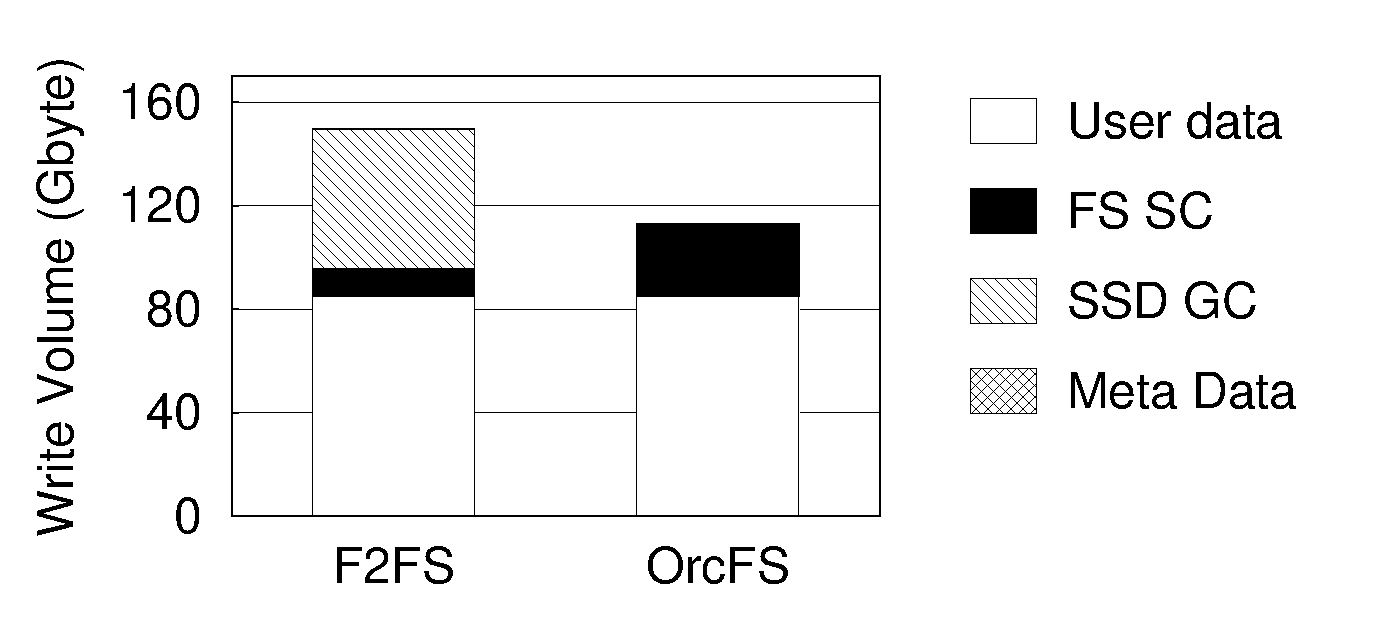
\includegraphics[width=3in]{./comp_gc/io_distribution.eps}
\caption{Total Write Volume Distribution (4 Kbyte buffered random
  write, Write volume generated by the application is 85 Gbyte,
  Section size of F2FS: 256 Mbyte)}
\label{fig:io_distribution}
%\vspace{-1.5em}
\end{center}
\end{figure}


\begin{comment}
  \begin{figure}[t]
  \begin{center}
  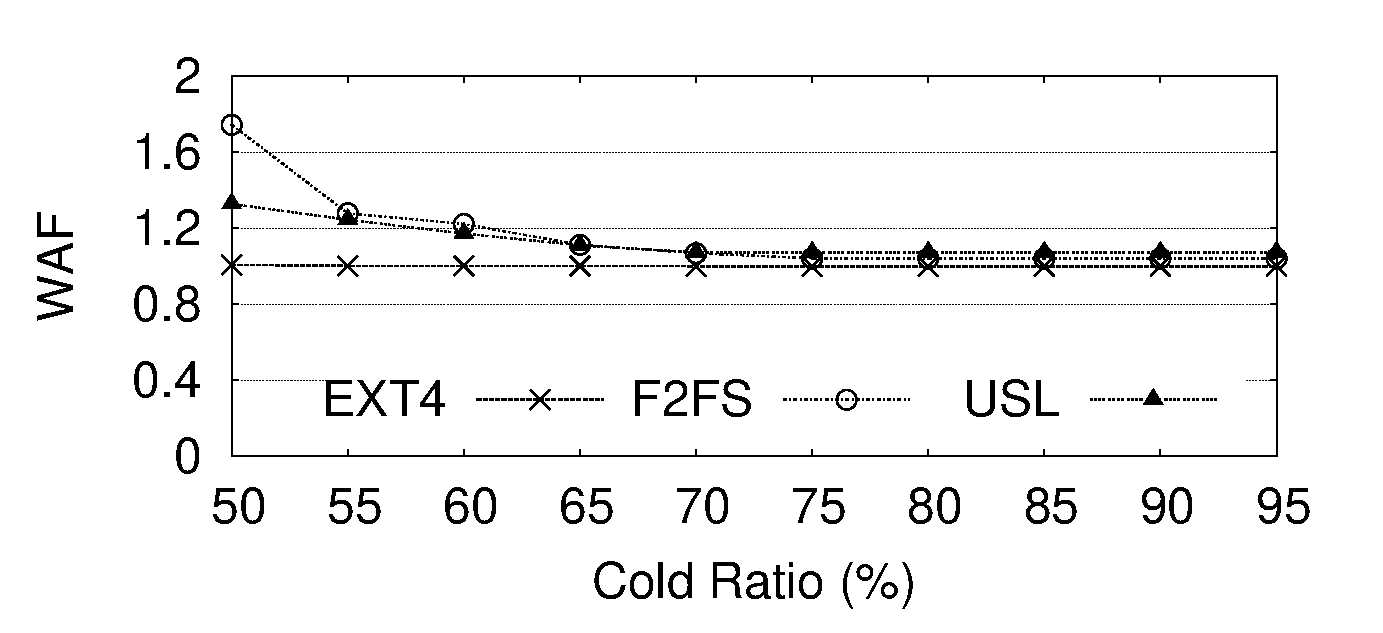
\includegraphics[width=3.2in]{./comp_gc/cold_ratio_waf.eps}
  \caption{WAF according to the Cold Data Ratio (The total size of
    cold data and hot data is 170 Gbyte, Section size of F2FS: 256
    Mbyte)}
  \label{fig:cold_ratio_waf}
%  \vspace{-1.5em}
  \end{center}
  \end{figure}
\end{comment}


\subsection{Block Patching Overhead}
\label{subsec:patching_overhead_test}

Depending on the nature of the workload, the space overhead of the
block patching can vary widely. We examine the block patching overhead
in three workloads which we have used in this study: random write,
varmail, and YCSB workload. Each of these workloads has widely
different access characteristics. YCSB benchmark uses log-structured
merge tree which flushes the dirty page cache entries in the unit of
tens of Mbyte. The overhead of block patching is negligible (0.3\%).
On the other hand, varmail workload frequently calls \texttt{fsync()}
to synchronize the updated file metadata to the storage. In this
workload, block patching entails 28\% overhead. For random write, the
block patching overhead is 2\%.

\begin{table}[t]
  \begin{center}
  \begin{tabular}{|c|c|c|c|} \hline
  Workload 							& Dummy Write	& Total Write	& Ratio 		\\ \hline\hline
  varmail	 (\cref{subsec:micro_bench})	& 514 MB		& 1.8 GB		& 28\%	\\ \hline
  YCSB (\cref{subsec:ycsb_bench})		& 196 MB		& 74 GB		& 0.3\%	\\ \hline
  Rand W (\cref{subsec:remove_gc_overhead}) & 2 GB		& 113 GB		& 2\%	\\ \hline
  \end{tabular}
  \end{center}
  \caption{Block Patching Overhead}
  \label{tab:block_patching}
\end{table}


\section{Related Works}
\label{sec:related_works}

\paragraph{Flash based File System: }
There are a number of efforts, such as YAFFS \cite{manning2010yaffs},
JFFS2 \cite{zhang2006implementation}, LogFS \cite{engel2005logfs}, and
UbiFS \cite{hunter2008brief}, to manage the raw Flash device on the
host side.  Since it does not have a Flash Translation Layer (FTL) in
the device, the host file system has to provide the mechanism for bad
block management, wear-leveling, and garbage collection. Moreover,
they only support one Flash memory device. 

FusionIO introduced Direct File System, DFS \cite{josephson2010dfs}
which is a file system for a high-performing SSD.  DFS keeps
Virtualized Flash Storage Layer to manage block allocation and inode
management that used to be the role of the file system. Because
DFS directly manages the mapping of the SSD, it does not suffer from
compound segment collection problem.

\paragraph{Reducing the Metadata Overhead:}

To relieve the burden of the device memory requirement, FSDV
(File System De-Virtualizer) \cite{zhangremoving} provides a way for
the host to manage the physical address mapping information. It
achieves to reduce the mapping table management overhead by removing
the logical to physical address mapping information on SSD.

Unlike FSDV which removed the overhead of device mapping information,
NVMKV \cite{nvmkv} removes the host side metadata management overhead
by replacing FTL commands with key-value operations. NVMKV uses
commands like atomic multiple-block \texttt{write}, \texttt{p-trim},
\texttt{exits}, and \texttt{iterate}, as the interface to the Flash
device.


\paragraph{Host Managed Storage System: }
ANViL \cite{anvil} lets the host modify logical-to-physical mapping
information on a device through new I/O interfaces. The host exploits
the given interfaces to remove the redundant data copy overhead. It
also provides useful features such as single journaling and file
snapshot to the system.

\paragraph{Compound Segment Collection:}
The compound segment collection problem on stacked log system is first
enlighted by Yang et al. \cite{yang2014don}. Since then Baidu
introduced SDF (Software-defined Flash) \cite{sdf}, Lee et
al. introduced AMF (Application Managed-Flash)
\cite{lee2016application}, and Zhang et al. proposed
ParaFS \cite{zhang2016parafs}.


AMF (Application Managed-Flash) \cite{lee2016application}, which is
based on F2FS \cite{lee2015f2fs}, exploits the fact that
log-structured applications always append the data to reduce the size
of metadata for Flash based storage. AMF modified the metadata area
of F2FS so that it is also managed in a log-structured manner; thus, it can
exploit the block mapping in the storage layer. Since both layers of
the file system and the Flash device can use block mapping, it gives a
partial solution to the compound segment collection problem.

ParaFS \cite{zhang2016parafs} acquires hardware information for the
storage to identify the number of channels the device has. ParaFS
exploits the information to distribute the data according to their
hotness and maximize the channel parallelism. It also implements
a coordinated garbage collection scheme and parallelism-aware scheduling
to solve the compound segment collection and load balancing.


\section{Conclusion}
\label{sec:conclusion}

Modern IO stacks are full of unnecessary redundancies with duplicate
efforts across the layers: the storage device, host file system and
even the application. To fully exploit the append-only and asymmetric
read/write latency nature of the Flash storage device, these three
layers endeavor to align their behavior to the physical
characteristics of the Flash storage. Each of these layers introduces
the level of indirection maintaining its address translation
information using log-structured file systems or using append-only
search structures such as log-structured merge tree. Subsequently, each
of the file system and the storage device reserves a certain fraction
of its space to consolidate the invalid blocks.  This duplicate
effort leads to the waste of the storage space, the increase in the
write-amplification and the performance degradation. In this work, we
propose OrcFS, Orchestrated File System, which orchestrates the
behavior of the Flash friendly file system and the flash storage,
respectively. OrcFS partitions the storage space into two regions and
assigns the management role of individual partitions to different
layers of the stack: the file system and the storage device. OrcFS fully
exploits the internal parallelism of the underlying flash storage
(multi-channel and multi-way) via making the unit of segment cleaning
equivalent to the superblock of the underlying Flash storage. Novel
Quasi-Preemptive Segment Cleaning algorithm effectively resolves the
excessive IO delay which may entail due to large segment cleaning unit
size.

The engineering achievement of the OrcFS is impressive.  It reduces the
device mapping table size to 1/465 and to 1/5 from the page mapping and
the smallest mapping table size proposed in the literature,
AMF, respectively.  Despite its minimal hardware resource
requirement, the OrcFS exhibits superior performance against EXT4 and
F2FS over page mapping based SSD in a broad range of workloads: 
synchronous random write dominant workload, \texttt{varmail} as well
as, append-only asynchronous write dominant workload such as YCSB.
Via eliminating the compound segment cleaning efforts in the
file system and the storage device, we eliminate 1/4 of the write
volume to the storage device leading to the roughly 30\% extension of
its lifespan.

% Acknowledgments
%\begin{acks}
%The authors would like to thank Dr. Maura Turolla of Telecom
%Italia for providing specifications about the application scenario.
%\end{acks}

\bibliographystyle{acmsmall}
\bibliography{ref}

% History dates: Received, Revised, Accepted
%\received{February 2007}{March 2009}{June 2009}

%\pagebreak
%\tableofcontents


\end{document}
